\section{Introduction}

%The Internet has crossed new frontiers with access to it getting faster and cheaper. New applications and services are being offered. Information and communication is of utmost importance during emergency response. The Internet plays a crucial role in enabling access to critical information that can save lives of people. Internet is now seen as critical infrastructure � enabling remote health care, education, employment, e-governance, digital economy, and social networks. 

%In the reality of today�s Internet, the vision of digital inclusion faces the challenge of a growing digital divide, i.e., a growing disparity between those with sufficient access to the Internet and those who cannot afford the access to universal services. 

The Internet has evolved into a critical infrastructure for education, employment, e-governance, remote health care, digital economy, and social media. However, Internet today is facing the challenge of a growing digital divide, i.e., an increasing disparity between those with and without Internet access. Access problems often stem from sparsely spread populations living in physically remote locations, since it is simply not cost-effective for Internet Service Providers (ISPs) to deploy the required infrastructure for broadband Internet access in these areas. Coupled with physical limitations of terrestrial infrastructures (mainly due to distance) to provide last mile access, remote communities also incur higher costs for connection between the exchange and backbone network when using wired technologies, because the distances are longer. A large exchange may accommodate many users and allow for competition between service operators; in contrast, a rural/remote broadband connection does not usually offer economies of scale, increasing the costs per user. 

This problem is widely and publicly recognized. For example, in 2012 9.1 million homes in Europe still did not have fixed broadband coverage, more than 90\% of which are in rural areas \cite{BROAD2012}. Achieving ubiquitous mobile broadband coverage is also currently seen as not feasible by major operators as direct investment in local infrastructure may be uneconomic.

Addressing digital exclusion due to socio-economic barriers is also important. The United Nations revealed the global disparity in fixed broadband access, showing that access to fixed broadband in some countries costs almost 40 times their national average income \cite{FILD2010}. This problem is also applicable to developed countries where many individuals find themselves unable to pass a necessary credit check or living in circumstances that are too unstable to commit to lengthy broadband contracts \cite{LCDNet}. A recent survey in Nottingham, UK \cite{NCC2012} revealed that affordability is cited as the primary barrier, explicitly so by over 22.7\% of digitally excluded in the age of 16-44 years. 

We see enabling benevolence in the Internet (act of sharing resources) as a potential solution to solve the problem of digital exclusion caused due to socio-economic barriers. Lowest Cost Denominator Networking (LCDNet) \cite{LCDNet} is a new Internet paradigm that architects multi-layer resource pooling Internet technologies to support new low-cost access methods that could greatly reduce a network operator's direct investment in local infrastructure to support wider Internet access. LCDNet proposes to bring together several existing resource pooling Internet technologies to ensure that donors (users and network operators), who share their resources, are not affected and at the same time are incentivized for sharing their resources.  

Public Access WiFi Service (PAWS) \cite{PAWS} is based on LCDNet using a set of techniques that make use of the available unused capacity in home broadband networks and allowing Less-than-Best Effort (LBE) access to these resources \cite{LCDNet}. PAWS adopts an approach of community-wide participation, where broadband customers are enabled to donate controlled but free use of their high-speed broadband Internet by fellow citizens. Other initiatives have already explored sharing a user's broadband Internet connection via wireless (e.g., FON \cite{FON}). Although these methods are gaining worldwide acceptance, they are usually viewed as an extension of a user's paid service which is accessible only by other customers of the same service. In contrast, PAWS offers free access to essential services to all. 

To protect the consumer's paid service and the service provider revenue, it is essential to ensure that the guest user traffic does not impact perceived performance of the bandwidth donor (customer). The PAWS service is therefore constrained to offer a LBE access to network resources (lower quality compared to the standard Internet service offered to paying users). Various methods are being considered, including enabling LBE QoS (both in layers 2 and 3) in the network.

\begin{figure}[b]
\begin{center}
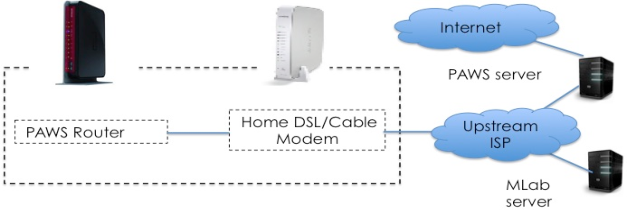
\includegraphics[width=1\linewidth]{paws.pdf}  
\caption{PAWS network.}
\label{fig:paws}
\end{center}
\end{figure}

PAWS is currently under deployment with 20 custom-made PAWS routers placed in a deprived community in Nottingham and another 10 routers in rural Scotland (Fig. \ref{fig:paws}). PAWS currently serves as a medium-scale open network measurement observatory in the UK allowing researchers to gather data about network availability, reachability, topology, security, and broadband performance from distributed vantage points in socio-economically deprived urban and rural areas. The PAWS deployment is essentially a crowd-shared access network (similar to FON) for under-privileged users in urban and rural communities. This provides the research community with a wealth of information on the needs of under-privileged users in terms of their access patterns and what do they use Internet access for. %The testbed also provides researchers the opportunity to understand behavioral patterns of home broadband users in terms of how do they share their home broadband networks with the public, e.g., how often do they switch off their home access points and when (day/time) do they switch it off. 
However, PAWS has faced ongoing deployment challenges, such as limited coverage, due to home user sharing patterns (i.e., home network users stop sharing their Internet connection for certain periods).

In this paper, we investigate the potential benefits of enabling PAWS or any crowd-shared wireless network as a crowd-shared wireless mesh network (WMN). Leveraging on the principles of software-defined networks (SDN), we perform a comparative study between PAWS and a crowd-shared WMN, considering the WMN managed by a centralized SDN controller with a global network view. To this end, we generate a model for home network user sharing patterns based on the router on/off periods captured from the PAWS deployment. Using simulations, we show that a crowd-shared WMN can achieve very high utilization of the shared bandwidth and can accommodate a significantly larger volume of guest user traffic compared to PAWS.

The remainder of the paper is organized as follows. In Section \ref{sec:architecture}, we discuss the management of the WMN and present techniques for guest user traffic redirection. In Section \ref{sec:evaluation}, we present our simulation environment and discuss the benefits of using a crowd-shared WMN for public Internet access. Finally, Section \ref{sec:conclusion} highlights our conclusions.
